\documentclass[letter]{article}
% Set target color model to RGB
\usepackage[inner=2.0cm,outer=2.0cm,top=2.5cm,bottom=2.5cm]{geometry}
\usepackage{setspace}
\usepackage[dvipsnames]{xcolor}
\usepackage{verbatim}
\usepackage{subcaption}
\usepackage{biblatex}
\usepackage{amsgen,amsmath,amstext,amsbsy,amsopn,tikz,amssymb,tkz-linknodes}
\usepackage{float}
\usepackage{fancyhdr}
\usepackage[colorlinks=true, urlcolor=blue,  linkcolor=blue, citecolor=blue]{hyperref}
\usepackage[colorinlistoftodos]{todonotes}
\usepackage{rotating}
\usepackage{booktabs}

\hypersetup{%
pdfauthor={Paul Shao},%
pdftitle={Worksheet},%
pdfkeywords={Tikz,latex,bootstrap,uncertaintes},%
pdfcreator={PDFLaTeX},%
pdfproducer={PDFLaTeX},%
}

\newcommand{\ra}[1]{\renewcommand{\arraystretch}{#1}}

\newtheorem{thm}{Theorem}[section]
\newtheorem{prop}[thm]{Proposition}
\newtheorem{lem}[thm]{Lemma}
\newtheorem{cor}[thm]{Corollary}
\newtheorem{defn}[thm]{Definition}
\newtheorem{rem}[thm]{Remark}
\numberwithin{equation}{section}

\newcommand{\homework}[5]{
   \pagestyle{myheadings}
   \thispagestyle{plain}
   \newpage
   \setcounter{page}{1}
   \noindent
   \begin{center}
   \framebox{
      \vbox{\vspace{2mm}
    \hbox to 6.28in { {\bf CSM 16A \hfill {\small #2}} }
       \vspace{6mm}
       \hbox to 6.28in { {\LARGE \hfill #1  \hfill} }
       \vspace{6mm}
       \hbox to 6.28in { {\it Term: {\rm #3} \hfill Name: \hspace{2cm}{\rm #4}}}
      \vspace{2mm}}
   }
   \end{center}
   \markboth{#5 -- #1}{#5 -- #1}
   \vspace*{4mm}
}

\newcommand{\problem}[1]{~\\\fbox{\textbf{Problem #1}}\hfill}
\newcommand{\subproblem}[1]{~\newline\textbf{(#1)}}
\newcommand{\D}{\mathcal{D}}
\newcommand{\Hy}{\mathcal{H}}
\newcommand{\VS}{\textrm{VS}}
\newcommand{\solution}{~\newline\textbf{\textit{(Solution)}} }

\newcommand{\bbF}{\mathbb{F}}
\newcommand{\bbX}{\mathbb{X}}
\newcommand{\bI}{\mathbf{I}}
\newcommand{\bX}{\mathbf{X}}
\newcommand{\bY}{\mathbf{Y}}
\newcommand{\bepsilon}{\boldsymbol{\epsilon}}
\newcommand{\balpha}{\boldsymbol{\alpha}}
\newcommand{\bbeta}{\boldsymbol{\beta}}
\newcommand{\0}{\mathbf{0}}

\newcommand{\sol}[1]{{\color{blue} \textbf{Solution: } #1}} % solutions in blue
\newcommand{\learning}[1]{{\color{ForestGreen} \textbf{Learning Goal: } #1}}
\newcommand{\note}[1]{{\color{purple} \textbf{Meta: } #1}} % notes in green
\newcommand{\answerbox}[1]{
   \noindent\fbox{
      \parbox{16cm}{
          \hspace{16cm}
          \vspace{#1}
      }
  }
}
\newcommand{\statement}[1]{
   \noindent\fbox{
      \parbox{16cm}{
          #1
      }
  }
}
\renewcommand{\note}[1]{}
\begin{document}
\homework{\textbf{Week 6 Worksheet \color{blue} Solutions}}{Designing Information Systems and Devices}{\textbf{Spring 2020}}{}{}
\problem{1: Kirchoff's Laws}
\\
\note{
    Make clear that the voltage divider equation relates the output voltage to the voltage at the input of the first resistor for the first part. Then, for the third part, show how having the second voltage divider attached to the Vmid of the first one invalidates the first part as a voltage divider.
}

\begin{enumerate}
    \item Here, you can see two standard voltage dividers. Find the voltage at the points $A$ and $B$ using standard nodal analysis techniques.\\
    \begin{circuitikz}
        \draw (0,-2)
            node[ground]{}
            (0,0) to[V=$V$] (0,-2)
            (0,0) to[R=$R_1$] (4,0)
            node[above] {$A$}
            to[R=$R_2$] (4,-2)
            node[ground]{};

        \draw (8,-2)
            node[ground]{}
            (8,0) to[V=$V$] (8,-2)
            (8,0) to[R=$R_3$] (12,0)
            node[above] {$B$}
            to[R=$R_4$] (12,-2)
            node[ground]{};
    \end{circuitikz}
    
    \sol{
    We can apply KCL at node $A$. We get:
    \begin{flalign*}
    & \frac{V_A - 0}{R_2} = \frac{V - V_A}{R_1} &\\
    & \implies \frac{R_1}{R_2}V_A = V - V_A &\\
    & \implies V_A (1 + \frac{R_1}{R_2}) = V &\\
    & \implies V_A \frac{R_1 + R_2}{R_2} = V &\\
    & \implies V_A = V \frac{R_2}{R_1 + R_2} &\\
    \end{flalign*}
    Similarly, for the second circuit, we have
    \begin{flalign*}
    & V_B = V \frac{R_4}{R_3 + R_4} &\\
    \end{flalign*}
    }
    
    \item Now, let us modify this circuit to add a second voltage divider stage starting at A. You can think of this as cascading 2 voltage dividers: one which which has an input of $V$ and an output of $V_A$, and a second one that has an input of $V_A$ and an output of $V_B$. Find the voltage at $B$ using nodal analysis.
    
    \begin{circuitikz}
        \draw (0,-2)
            node[ground]{}
            (0,0) to[V=$V$] (0,-2)
            (0,0) to[R=$R_1$] (4,0)
            node[above] {$A$}
            to[R=$R_2$] (4,-2)
            node[ground]{};
        \draw (4,0)
            to[R=$R_3$] (8,0)
            node[above] {$B$}
            to[R=$R_4$] (8,-2)
            node[ground]{};
    \end{circuitikz}
    
    \sol{
    We can apply KCL at node $A$ and at node $B$. We get the equations:
    \begin{flalign*}
    & \frac{V - V_A}{R_1} + \frac{0 - V_A}{R_2} = \frac{V_A - V_B}{R_3} &\\
    & \frac{V_A - V_B}{R_3} = \frac{V_B - 0}{R_4} &\\
    \end{flalign*}
    
    We can simplify these equations to give us
    \begin{flalign*}
    & \frac{V}{R_1} - \frac{V_A}{R_1} - \frac{V_A}{R_2} = \frac{V_A}{R_3} - \frac{V_B}{R_3} &\\
    & \implies \frac{V_B}{R_3} + \frac{V}{R_1} = \frac{V_A}{R_1} + \frac{V_A}{R_2} + \frac{V_A}{R_3} &\\
    & \implies \frac{V_B}{R_3} + \frac{V}{R_1} = V_A (\frac{1}{R_1} + \frac{1}{R_2} + \frac{1}{R_3}) &\\
    & \frac{V_A}{R_3} - \frac{V_B}{R_3} = \frac{V_B}{R_4} &\\
    & \implies \frac{V_A}{R_3} = \frac{V_B}{R_3} + \frac{V_B}{R_4} &\\
    & \implies V_A = V_B R_3 (\frac{1}{R_3} + \frac{1}{R_4}) &\\
    \end{flalign*}
    
    Combining these 2 equations, we get:
    \begin{flalign*}
    & \frac{V_B}{R_3} + \frac{V}{R_1} = V_B R_3 (\frac{1}{R_3} + \frac{1}{R_4}) (\frac{1}{R_1} + \frac{1}{R_2} + \frac{1}{R_3}) &\\
    & \implies \frac{V_B}{R_3} + \frac{V}{R_1} = V_B R_3 (\frac{1}{R_3} + \frac{1}{R_4}) (\frac{1}{R_1} + \frac{1}{R_2} + \frac{1}{R_3}) &\\
    & \implies \frac{V}{R_1} = V_B R_3 (\frac{1}{R_3} + \frac{1}{R_4}) (\frac{1}{R_1} + \frac{1}{R_2} + \frac{1}{R_3}) + \frac{V_B}{R_3} = V_B (R_3 (\frac{1}{R_3} + \frac{1}{R_4}) (\frac{1}{R_1} + \frac{1}{R_2} + \frac{1}{R_3}) + \frac{1}{R_3}) &\\
    & \implies V_B = \frac{V}{R_1} / (R_3 (\frac{1}{R_3} + \frac{1}{R_4}) (\frac{1}{R_1} + \frac{1}{R_2} + \frac{1}{R_3}) + \frac{1}{R_3})  &\\
    \end{flalign*}
    }
    
    \item Compare your answer with what you get when you multiplying the amplification factors of each individual voltage divider. Are they the same or different? Does this surprise you? Why or why not?

    \note{
    If students don’t entirely see why you can’t use the voltage divider twice, try redrawing the circuit. You can illustrate how R3 and R4 are in series, but both are in parallel with R2.
    }
    
    \sol{
    They are clearly not the same! The next part explains why.
    
    What we see here is called "loading". Ideally, we would like to be able to stack voltage dividers like this in order to cascade their effects. However this does not work because by adding the second circuit, we are changing what the first one does. In particular, the second circuit will draw some current from the first circuit. We can see this difference if we zoom in on the node A. In part (a), we had the following picture:
    
    \begin{circuitikz}
        \draw (0,0)
            (0,0) to[R=$R_1$, i=$i_1$] (4,0)
            node[above] {$A$}
            to[R=$R_2$, i=$i_2$] (4,-2)
            node[ground]{};
    \end{circuitikz}
    \\
    And we were able to say that $i_1 = i_2$, because they are the only currents at node $A$. But after adding the second voltage divider stage, the picture now looks like this:
    
    \begin{circuitikz}
        \draw (0,0)
            (0,0) to[R=$R_1$, i=$i_1$] (4,0)
            node[above] {$A$}
            to[R=$R_2$, i=$i_2$] (4,-2)
            node[ground]{}
            (4,0) to[short, i=$i_B$] (6,0);
    \end{circuitikz}
    \\
    And so the KCL equation we wrote at node $A$ is no longer valid. \\
    Voltage dividers "divide" the voltage between two resistors in series. However, when we add the second voltage divider, $R_1$ and $R_2$ can't be said to be in series anymore. 

    Think about the conditions under which the impact of cascaded voltage dividers can be calculated by simply multiplying the two ratios. We will learn how to do that later in lecture with a special circuit element which helps us "modularize" the circuit. 
    }
\newpage
\problem{2: Power}
\\
% Lydia Lee, lydia.lee@berkeley.edu

\note{
    For an arbitrary circuit element
    \begin{center}
        \begin{circuitikz}
            \ctikzset{resistor = european}
            \draw
            (0,0) to[R, v=$V_\text{element}$, i=$I_\text{element}$] ++(3,0);
        \end{circuitikz}
    \end{center}
    we can calculate the power it dissipates (i.e. the power it consumes) with the expression $$P_\text{element} = I_\text{element}V_\text{element}$$
}

\begin{enumerate}
\item\label{ques:resistor_expressions}{
    For resistors (and resistors only), we can relate the voltage drop across the resistor and the current passing through the resistor with Ohm's Law: $$V_R = I_RR$$
    \begin{center}
        \begin{circuitikz}
            \draw
            (0,0) to[R=$R$, v=$V_R$, i=$I_R$] ++(3,0);
        \end{circuitikz}
    \end{center}
    Find an expression for the power dissipated by the resistor in terms of the following:
    \begin{enumerate}
        \item $V_R$ and $I_R$
        \item $V_R$ and $R$
        \item $I_R$ and $R$
    \end{enumerate}
}

\note{

    Starting with the expression for power
    $$P_R = I_RV_R$$
    we manipulate Ohm's Law to find appropriate substitutions for the terms we can't use. In particular,
    \begin{align*}
        V_R &= I_RR\\
        I_R &= \frac{V_R}{R}
    \end{align*}
    From this we can also get
    \begin{align*}
        R &= \frac{V_R}{I_R}
    \end{align*}
    but in this case we don't actually need it.
}

\sol{

    \begin{enumerate}
        \item $I_RV_R$
        \item $\frac{V_R^2}{R}$
        \item $I_R^2R$
    \end{enumerate}
}

For the rest of this question, use the circuit below:
\begin{center}
    \begin{circuitikz}
    \draw
    (0,0) coordinate (BASE)
        to[I,l=$I_S$] ++(0,4)
        to[short] ++(1,0) coordinate (LHS)
    (LHS) to[short] ++(0,.5)
        to[R=$2\si{\ohm}$,l=$R_1$] ++(3,0)
        to[short] ++(0,-.5) coordinate (RHS)
    (LHS) to[short] ++(0,-.5)
        to[R=$2\si{\ohm}$, l=$R_2$] ++(3,0)
        to[short] (RHS)
    (RHS) to[short] ++(1,0) coordinate (TOPLEFT)
        to[R=$6\si{\ohm}$, l=$R_3$] (TOPLEFT |- BASE)
    (TOPLEFT) to[short] ++(2,0) coordinate (TOPRIGHT)
        to[R=$6\si{\ohm}$, l=$R_4$] (TOPRIGHT |- BASE)
        to[short] (BASE);
\end{circuitikz}
\end{center}
\item\label{ques:parallel}{
    Which individual components have the same magnitude voltage drop across them?
}

\sol{
    
    $R_1$ and $R_2$ are in parallel and so see the same voltage drop as one another.

    $R_3$ and $R_4$ are also in parallel and experience the same voltage drop as one another.
}

\item\label{ques:power_parallel}{
    Under what condition(s) will $R_1$ and $R_2$ dissipate the same amount of power?
}

\sol{

    We know $$P=IV$$ and that $R_1$ and $R_2$ have the same voltage drop across them. In order to dissipate the same amount of power, the two need to have equal current flowing through them in the same direction. Manipulating Ohm's Law, we get 
    $$I_1 = \frac{V}{R_1}, I_2 = \frac{V}{R_2}$$
    For these to be equal, $R_1$ must be equal to $R_2$. Alternatively, we can go straight to the expression for resistor power
    $$P_R = \frac{V_R^2}{R}$$
    and see from here that the resistances must be the same for the two to dissipate the same amount of power.
}

\item\label{ques:power_resistors}{
    Use the following values and calculate the amount of power consumed by each of the resistors $R_1, R_2, R_3,$ and $R_4$.
    \begin{center}
        \begin{tabular}{|c|c|c|}
            \hline
            Component & Value & Units\\\hline
            $R_1, R_2$ & 2 &$\si{\ohm}$\\\hline
            $R_3, R_4$ & 6 & $\si{\ohm}$\\\hline
            $I_S$ & 1 & $\si{\ampere}$\\\hline
        \end{tabular}
    \end{center}
}

\note{
    
    Ideally by this point students are comfortable with parallel/series combinations of resistors. You should be prepared to work out the problem in full rigor if your students ask.
}

\sol{
    
    To find the power dissipated by a resistor, we can use any of the following:
    \begin{align*}
        P &= IV\\
            &= \frac{V^2}{R}\\
            &= I^2R
    \end{align*}
    Because we're already given the resistance, we can either find the voltage drop across each of the resistors or the current flowing through them. Redrawing the circuit with the numerical values labeled:
    \begin{center}
        \begin{circuitikz}
    \draw
    (0,0) coordinate (BASE)
        to[I,l=$1\si{\ampere}$] ++(0,4)
        to[short] ++(1,0) coordinate (LHS)
    (LHS) to[short] ++(0,.5)
        to[R=$2\si{\ohm}$] ++(3,0)
        to[short] ++(0,-.5) coordinate (RHS)
    (LHS) to[short] ++(0,-.5)
        to[R=$2\si{\ohm}$] ++(3,0)
        to[short] (RHS)
    (RHS) to[short] ++(1,0) coordinate (TOPLEFT)
        to[R=$6\si{\ohm}$] (TOPLEFT |- BASE)
    (TOPLEFT) to[short] ++(2,0) coordinate (TOPRIGHT)
        to[R=$6\si{\ohm}$] (TOPRIGHT |- BASE)
        to[short] (BASE);
\end{circuitikz}
    \end{center}
    \textbf{Current Solution:}
    We know from part \ref{ques:power_parallel} that $R_1$ and $R_2$ will have the same amount of current flowing through them, i.e. the $1\si{\ampere}$ is evenly divided between them. The same goes for $R_3$ and $R_4$.
    \begin{align*}
        P_{R_1, R_2} &= \left(\frac{1}{2}\si{\ampere}\right)^2 \cdot 2\si{\ohm}\\
            &= 0.5 \si{\watt}\\
        P_{R_3, R_4} &= \left(\frac{1}{2}\si{\ampere}\right)^2 \cdot 6\si{\ohm}\\
            &= 1.5 \si{\watt}
    \end{align*}

    \textbf{Voltage Solution:}
    Using parallel resistor combinations, we can combine the two $2\si{\ohm}$ and combine the two $6\si{\ohm}$ resistors to get the following:
    \begin{center}
        \begin{circuitikz}
    \draw
    (0,0) coordinate (BASE)
        to[I,l=$1\si{\ampere}$] ++(0,4)
        to[R=$1\si{\ohm}$,v=$V_{1,2}$] ++(3,0) coordinate (RHS)
        to[R=$3\si{\ohm}$,v=$V_{3,4}$] (RHS |- BASE)
        to[short] (BASE);
\end{circuitikz}
    \end{center}
    We're given a current source, so we can use Ohm's law to find $V_{1,2}$ and $V_{3,4}$:
    \begin{align*}
        V_{1,2} &= 1\si{\ampere}\cdot1\si{\ohm}\\
            &= 1\si{\volt}\\
        V_{3,4} &= 1\si{\ampere}\cdot3\si{\ohm}\\
            &= 3\si{\volt}
    \end{align*}
    and from here
    \begin{align*}
        P_{R_1, R_2} &= \frac{V_{1, 2}^2}{2\si{\ohm}}\\
            &= \frac{(1\si{\volt})^2}{2\si{\ohm}}\\
            &= 0.5\si{\watt}\\
        P_{R_3, R_4} &= \frac{V_{3, 4}^2}{6\si{\ohm}}\\
            &= \frac{(3\si{\volt})^2}{6\si{\ohm}}\\
            &= 1.5\si{\watt}
    \end{align*}
}

\item\label{ques:power_source}{
    How much power does the current source consume? \textit{Hint: Consider the conservation of energy.}
}

\note{   
    Again, be prepared to work this out in full rigor if your students ask.
}

\sol{
    Because of the conservation of energy (and by proxy power because $P = \frac{dE}{dt}$), we know all the power the resistors dissipate must be generated by the current source. Using our answers from part \ref{ques:power_resistors}:
    \begin{align*}
        P_{I_S} + P_{R_1} + P_{R_2}+ P_{R_3} + P_{R_4} &= 0\si{\watt}\\
        P_{I_S} &= -P_{R_1} - P_{R_2}- P_{R_3} - P_{R_4}\\
            &= -(0.5\si{\watt} + 0.5\si{\watt} + 1.5\si{\watt} + 1.5\si{\watt})\\
            &= -4\si{\watt}
    \end{align*}

    Note the sign! Negative power indicates that a component is dissipating negative power, i.e. that it's generating power.
}
\end{enumerate}
\newpage
\problem{3: Rubik's Cube (With Resistors!)}
\\
In this question, we will guide you through how to apply nodes and resistance equivalence to solve a complex resistor network (like the cubic one above, assuming all resistors are identical with a resistance of $R$) and find the equivalent resistance between the top back left node and the bottom front right node. \\
\note{For this question, encourage the students to follow through the questions and apply nodal analysis and equivalent resistance along the way. Assure them that with the symmetrical nature of this cubic network, the result will appear less complicated than they expect.}

\begin{figure}[H]
    \centering
    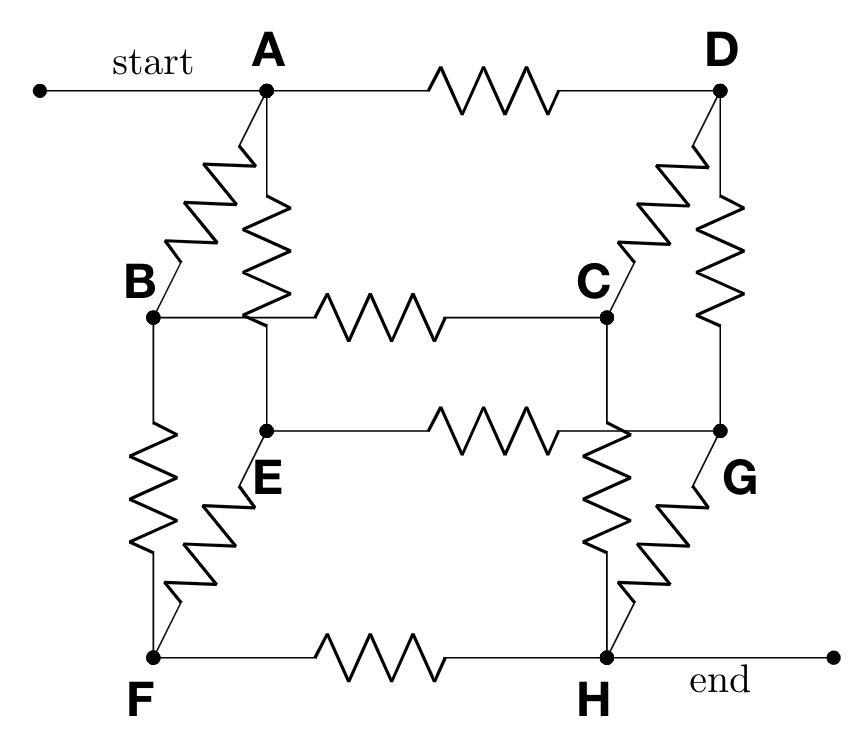
\includegraphics[scale=0.45]{../labeled.png}
    \caption{3D View of the Resistor Network}
\end{figure}

\begin{figure}[H]
    \centering
    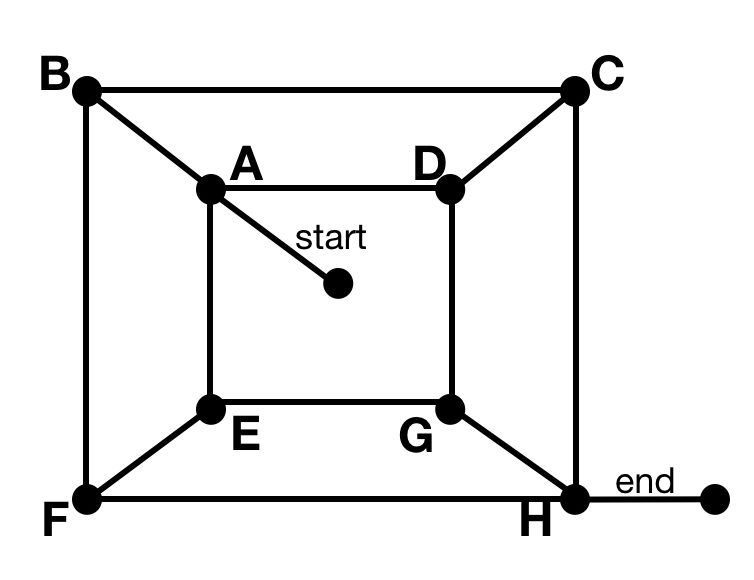
\includegraphics[scale=0.45]{../flattened.png}
    \caption{Flattened View of the Resistor Network, \\ where each segment between 2 nodes has a resistance of $R$}
\end{figure}

\begin{enumerate}
    \item As daunting as this question looks, fortunately we have the power of nodal analysis on our side! To get started, group the vertices from $B$ through $H$ based on the \textbf{distances of the shortest paths} along the edges of the cube starting from $A$. For example, the distance of the shortest path from $A$ to the bottom front left vertex will be 2 (assuming each edge of the cube is 1 unit long). \\
    \note{Make sure to clarify to the students that shortest path always starts from $A$ (as our point of departure) and must go along the edges of the cube.} \\
    \sol{
        Starting from the vertex $A$, we can see that:
        $B$, $D$, and $E$ are all 1 unit away from $A$, while $F$, $G$, abd $C$ are 2 units away from $A$, and $H$ (the endpoint) is 3 units away from $A$.
    }
    \item Now, consider the group of all the vertices $v_i$ that are 1 unit away from $A$ (the starting node in the top back left) and the resistors in and between these pairs of nodes ($v_i$, $A$). How are they related to each other (Hint: think in terms of equivalent resistance)? \\
    \note{For this part, encourage the students to think in terms of potential differences. Use the following scenario as an example to provide them with some helpful hints: \\
    Suppose I have 2 pairs of nodes $(A, B)$ and $(C, D)$, both pairs have the same resistances between them $R_{A-B} = R_{C-D}$. What can we conclude about the potential differences ($V_{A-B}, V_{C-D}$) of both pairs?
    } \\
    \sol{Based on our labeling convention in the previous part, the nodes that are 1 unit away from $A$ are $B$, $D$, and $E$. Since all these nodes are of the same distance away from the starting node $A$, and the resistance between these nodes and $A$ is the same ($R$), the potential differences between $A$ and these nodes are \textbf{all the same}! This means that the 3 resistors between $A$ and the nodes that are 1 unit away from it are in parallel.}
    \item Now, consider the group of all the vertices $v_j$ that are 2 units away from $A$. Call it Group II. Let the group in the previous part be Group I. How many edges lead from a vertex in Group I to a vertex in Group II (how many resistors are involved in this case)? \\
    \sol{To count how many edges lead from a vertex in Group I to a vertex in Group II, we can begin with any vertex from the set $\{B, D, E \}$ and count the number of distinct edges that lead from it 1 unit farther away from $A$. As we can see in the cube above, for each vertex $v_i$ in Group I, there are exactly 2 distinct edges that lead to a vertex 1 unit farther away from $A$. So, there are $3 \times 2 = 6$ such edges in total. Since each edge contains a resistor, there are 6 resistors involved in total.}
    \item How are Group I and Group II related with each other? Is there anything we can do to simplify the resistor network so far? \\

    \note{When teaching, encourage the students to think about the following questions before working on this part:

    \begin{itemize}
        \item What happens if you merge the vertices(nodes) with the same potentials into one?
        \item How can we apply this to Group I, Group II and the resistors involved in both groups?
    \end{itemize}
    }

    \sol{
        When we have nodes with the same potential, if we merge them into one, the overall potential difference between the merged endpoint and $A$ still remains the same. This implies that merging all nodes with the same potential into one junction won't affect the overall structure or resistance of this resistor network!
        
        Since nodes in Group II are 1 unit away from the nodes in Group I, and similarly, all resistors in and between are in parallel as well, we can merge their start nodes and end nodes into a single junction as well! Therefore, the overall resistors between the vertices in Group I and $A$ are in series with those between the vertices in Group I and the vertices in Group II. So essentially, we have 3 resistors (from Group I) in parallel, and overall in series with 6 resistors (between Group I and Group II) in parallel.
    }
    \item Finally, How far away is $H$ (the ending node) from $A$ (the starting node)? How many edges are there that lead from the nodes in Group II to $H$? Using equivalent resistance, is there anyway we can simplify all the circuits along the edges from the nodes in Group II to $H$? (Hint: think in terms of symmetry and what you've found in part (b)) \\
    \sol{Here comes the symmetrical beauty that underlines this cubic network! If we rotate the entire cubic resistor network by 180 degrees about the space diagonal from $A$ and $H$, we will exactly end up with $A$ swapped with $H$. What this really means is that all the edges that lead from the vertices in Group II to $H$ are equivalent to the edges that first extend 1 unit away from $A$ in part (b)! This further implies that the 3 resistors along these edges are in parallel again (as we converge back onto one end node)!}
    \item Combining all your findings together, what is the overall resistance between the starting node on the top back left and the ending node on the bottom front right in this cubic resistor network? \\
    \note{For the final part, encourage the students to try "flattening" the 3D resistor network onto a plane. Make sure to bring up how they can apply all the resistance equivalence they've discovered over the previous parts to map out all the resistors based on the nodes and their shortest distances from $A$.} \\
    \sol{
    Let's recap what we've known so far, go through the groups of nodes and the resulting junctions that we merged from the previous parts.
    \begin{enumerate}
        \item Starting from $A$, we have 3 resistors in parallel. Over a distance of 1 unit, we reach the nodes $B, D, E$ in Group I. By the equivalent resistance in a parallel circuit, the overall resistance of these 3 resistors is $\frac{R}{3}$.
        \item Between Group I and Group II, since the distance in and between the vertices from the 2 groups is the same (= 1 unit), and each edge carries the same resistor, this means all edges share the same potentials, therefore, we can merge all the start nodes into one junction $T_0$, and all the end nodes into another junction $T_1$. $T_0$ will contain the vertices $B, D, E$, and $T_1$ will contain the vertices $C, F, G$. Overall between the merged junctions, we have 6 edges (or resistors) in parallel with each other. Therefore, the overall resistance of this part will be $\frac{R}{6}$
        \item Between Group II and the end node $H$, by symmetry from part(e), we can apply what we've done exactly for Group I and $A$. Hence, the overall resistance of this part will be again $\frac{R}{3}$.
        \item All these 3 parts are in series with each other (from $A$ to $H$), hence, by the equivalent resistance of a series circuit, the total resistance between $A$ and $H$ is equal to 
        $$ \frac{R}{3} + \frac{R}{6} + \frac{R}{3} = \frac{5}{6}R$$
        Again, with the power of nodal analysis and equivalent resistance, anything is possible! $\square$
    \end{enumerate}
    }
\end{enumerate}
\newpage
\problem{4: Superposition}
\\
\begin{enumerate}
    \item{ 
    
    Solve the following circuit for $V_x$ using nodal analysis. Let $R_1 = 10 \Omega$, $R_2 = 5 \Omega$, $R_3 = 2 \Omega$, $V_1 = 7 V$, and $I_1 = 6 A$.
    
    %Full circuit for this question
        \begin{center}
        \begin{circuitikz}
    
        \draw(0,4)
        to[R, l=$R_1$] ++(0,-2)
        %to node[left] {$V_1$} ++(0,0)
        to[V_=$V_1$] ++(0,-2)
        to[short] node[ground] {} ++(0,-1);
        
        \draw(2,4)
        to[short, i=$I_2$] ++(-2, 0);
        
        \draw(2,4)
        to[short, i=$I_3$] ++(2, 0);
        
        \draw(2,4)
        to node[above] {$V_x$} ++(0,0)
        to[I, l= $I_1$, invert] ++(0, -2)
        to node[left] {$V_a$} ++(0,0)
        to[R, l = $R_2$] ++(0, -2)
        to[short] ++(-2,0);
        
        \draw(4, 4)
        to[cV, l = $2I_2$] ++(0,-2)
        to node[left] {$V_b$} ++(0,0)
        to[R, l=$R_3$] ++(0,-2)
        to[short] ++(-2, 0);
        
        \end{circuitikz}
        \end{center}
    
    }

    \textbf{Note}: The diamond-shaped element in the circuit above represents a dependent voltage source. Specifically for this question, the amount of voltage it supplies depends on the current $i_2$: $V_{\text{dependent}} = 2i_2$.
    
    \note{
    
    Prerequsities: Understanding of linearity and superposition, and some familiarity with the idea of a voltage source supplying 0 volts or a current source supplying zero amps.
    Ensure that the students know what it means to 'turn off' a source (e.g. turning off a voltage source converts it into a wire).

    Clarify that the dependent source is a voltage source, not a current source. The value of the dependent voltage source is $V = 2I_2$. We can identify it is a voltage source because it has a $+$ and $-$ symbol, rather than a current arrow $\uparrow$.
    }
    
    \sol{
    Let us examine the case in which we see all currents flowing OUT of $V_x$:
    
    For the current flowing through $R_1$, $I_2$, we need to use Ohm's law. We know easily that above $R_1$ the voltage is $V_x$, as it is connected to the same node. Beneath, we have a voltage gain of $V_1$ from ground. (Remember, voltage sources power voltage differences rather than absolute values).
    Thus we have
    
    $$
    I_2 = \frac{V_x - V_1}{R_1}
    $$
    
    Since we're setting all currents as going out of $V_x$, we'll say the current going out on the branch with $I_1$ as $-I_1$. 
    
    Finally, the branch with dependent sources. The easiest way to find the current, again, is using the resistor $R_3$ and finding the current going through it. While the bottom terminal is connected to ground, what is the top terminal? 
    Say we followed the wire down from $V_x$. Then, when we cross the dependent voltage source, since sources power differences in voltage, we can say the voltage below it is equal to $V_b = V_x - 2I_2$.
    
    Thus, current through $R_3$, $I_3$ is 
    
    $$I_3 = \frac{V_x - 2I_2}{R_3}$$.
    
    We have the sum of currents equal to 0, as they are all going out.
    
    Thus,
    
    $$I_2 + (-I_1) + I_3 = 0$$
    $$\frac{V_x - V_1}{R_1} = I_1 - \frac{V_x - 2I_2}{R_3}$$
    
    Where $I_2$ is known. Thus we can solve this equation! Plugging in numbers,
    
    $$I_2 = \frac{V_x - 7}{10}$$
    $$\frac{V_x - 7}{10} = 6 - \frac{V_x - 2I_2}{2}$$
    $$\frac{V_x - 7}{10} = 6 - \frac{V_x - \frac{V_x - 7}{5}}{2}$$
    $$\frac{V_x - 7}{5} = 12 - V_x - \frac{V_x - 7}{5}$$
    $$V_x = 12$$
    
    }
    
    \item{
    Now solve the same circuit for $V_x$ using superposition. Please note that only \textbf{independent voltage/current sources} can be removed when using superposition.
    }

    \note{
        Make sure students understand how to nullify voltage / current sources when using superposition, and why they are short / open circuits.
    }
    
    \sol{
    
    Superposition circuit when removing the current source
        \begin{center}
        \begin{circuitikz}
    
        \draw(0,4)
        to[R, l=$R_1$, v=$ $] ++(0,-2)
        to[V_=$V_1$] ++(0,-2)
        to[short] node[ground] {} ++(0,-1);
        
        \draw(2,4)
        to[short, i=$I_2$] ++(-2, 0);
        
        \draw(2,4)
        to[short, i=$I_3$] ++(2, 0);
        
        \draw(2,4)
        to node[above] {$V_x$} ++(0,0)
        to[short, *-o] ++(0, -1);
        
        \draw(2,2)
        to node[right] {$V_a$} ++(0,0)
        to[R, l = $R_2$, v^<=$ $, *-o] ++(0, -2)
        to[short] ++(-2,0);
        
        \draw(4, 4)
        to[cV, l = $2I_2$] ++(0,-2)
        to node[right] {$V_b$} ++(0,0)
        to[R, l=$R_3$, v=$ $] ++(0,-2)
        to[short] ++(-2, 0);
        
        \end{circuitikz}
        \end{center}
    Setting this up, we get three equations, for $V_a$ we get:
    \[V_a = 0\]
    Next, lets observe the value of $I_2$ so that we can use that with the dependent source:
    \[I_2 = \frac{V_x - V_1}{R_1}\]
    Using this, we can now express the difference of voltage over the dependent source, i.e.:
    \[V_x - V_b = 2I_2 = 2\frac{V_x - V_1}{R_1}\]
    Next we note that in this version, that the current doesn't split anywhere, so $I_2 = -I_3$. So, we can find the voltage drop over $R_3$ as follows:
    \[\frac{0 - V_b}{R_3} = I_3 = -I_2 = -\frac{V_x - V_1}{R_1}\]
    
    So, repeating the above, our three equations are:
    \begin{align}
        V_a = 0 \\
        V_x - V_b = 2\frac{V_x - V_1}{R_1}\\
        \frac{0 - V_b}{R_3} = -\frac{V_x - V_1}{R_1}
    \end{align}
    %%%%%%
    %YOOOO dont forget to fix this:
    %%%%%%
    Superposition circuit while removing the voltage source
        \begin{center}
        \begin{circuitikz}

        \draw(0,4)
        to[R, l=$R_1$, v=$ $] ++(0,-2)
        to[short] ++(0,-2)
        to[short] node[ground] {} ++(0,-1);

        \draw(2,4)
        to[short, i=$I_2$] ++(-2, 0);

        \draw(2,4)
        to[short, i=$I_3$] ++(2, 0);

        \draw(2,4)
        to node[above] {$V_x$} ++(0,0)
        to[I, l= $I_1$, invert] ++(0, -2)
        to node[right] {$V_a$} ++(0,0)
        to[R, l = $R_2$, v^<=$ $] ++(0, -2)
        to[short] ++(-2,0);

        \draw(4, 4)
        to[cV, l = $2I_2$] ++(0,-2)
        to node[right] {$V_b$} ++(0,0)
        to[R, l=$R_3$, v=$ $] ++(0,-2)
        to[short] ++(-2, 0);

        \end{circuitikz}
        \end{center}

    Now, we will find the equivalent three equations for this form. Starting again with the voltage drop over $R_2$, we have:
    $$ \frac{0 - V_a}{R_2} = I_1 $$
    Next, again, let's find I_2:
    $I_2 = \frac{V_x - 0}{R_1} = \frac{V_x}{R_1}$
    Using this, we can find the difference over the dependent source:
    \[ V_x - V_b = 2I_2 = 2\frac{V_x}{R_1} \]
    Finally, we can express the voltage drop over $R_3$ via KCL:
    \[ I_1 = I_2 - I_3 = \frac{V_x}{R_1} - I_3 = \frac{V_x}{R_1} + \frac{0 - V_b}{R_3}\]
    We now again have three equations as follows:
    \begin{align}
        \frac{0 - V_a}{R_2} = I_1 \\
        V_x - V_b = 2\frac{V_x}{R_1}\\
        I_1 = \frac{V_x}{R_1} + \frac{0 - V_b}{R_3}
    \end{align}
    Now, we just plug in the numbers we have into our 6 numbered equations, and add up the values for matching voltages, and as a result we get:\\
    
    For nulling the current source:
    $$-V_b = \frac{2(V_x - 7)}{10}$$
    %https://www.sharelatex.com/project/59a8a8e71dc5c27add7c6b78
    $$V_x + \frac{2(V_x - 7)}{10} = 2\frac{V_x - 7}{10}$$
    $$V_x = 0$$
    
    For nulling the voltage source:
    $$6 = \frac{V_x}{10} - \frac{V_b}{2}$$
    $$-V_b = 12 - \frac{V_x}{5}$$
    $$V_x - 12 + \frac{V_x}{5} = 2\frac{V_x}{10}$$
    $$V_x = 12$$
    
    Then, adding the two values for $V_x$ together,
    $$0 + 12 = 12$$
    
    We have verified that the answer we get for superposition is the same as the answer we get using nodal analysis.
    
    }
    
    \end{enumerate}
\end{document}